%==================================================================
\chapter{Methodology} \label{appendix-methodology}
%==================================================================

% \epigraph{One of the very important components in the urban and agricultural land use model is the so-called \gls{bid-rent curve}. Regional and urban economists, city planners, and economic geographers have used this curve extensively as an analytical device.}{Yeung-Nan Shieh \cite{shiehWilhelmLaunhardtBidRent2004}}
 % \epigraph{It may be tempting to specify an aggregate production function that directly relates primary factors to final output, as is customary in much economic analysis. This standard simplification is often inadequate, however, because cities are characterized by increasing returns to scale, and how such increasing returns are generated has potentially important policy implications. In particular, detailed assumptions are needed about labor, the nature of products, the production function of individual firms, the input-output structure that links firms, and how firms compete.}{Spence et al \cite{spenceUrbanizationGrowth2009}}
 % TODO ADD THE PURPOSES OF MODELLING NOTE TO DISCUSSION OF HOW  WE ARE USING ABMS

% SUMMARIZE: WE ARE MODELLING THE RELATIONSHIP BETWEEN FINANCIALIZATION AS GRAWTH VALUE CAPTURES AND PRODUCTION IN CITIES TO DO THIS WE  BUILD ABM

% ROOTED IN NEOCLASSICAL AND CLASICAL (MOVE THAT SECTION UP??) 

% ABM ADDS WHAT?? GO INTO HISTORY OF ABM AND THEN HOW YOU USE IT TO MODEL THAT ASPECTS YOU HAVE INTRODUCED IN EARLIAR SECTIONS

We are modeling the relationship between financialization and the production of value in models. To do this we combine a spatially explicit agent-based land market model, with an equilibrium assumption about rent and an equation-based model of urban production. By integrating these three pieces, which are traditionally studied separately, this work combines elements of classical rent theory and neoclassical distribution theory with agent-based modeling. 

We employ equilibrium arguments derived from models of optimizing agents, who make decisions at the margin,  with an agent-based model (ABM) in which agents make periodic discrete choices among a small set of alternatives. We combine coarse generalizations about long-term agglomeration effects with fine-grained housing and financial market processes. We examine in moderate detail how financial decisions affect home ownership, while black-boxing 
the transmission of agglomeration effects through firms from aggregate productivity gains to population growth. 
% None of these represent methodological transgressions although the combinations may be unusual. 
% The methodological questions that this combination raise are interesting and we get additional insight into the financialization of housing markets by examining them further.

% We begin by reviewing the modeling paradigms, then discuss in some detail the relationship between analytic neoclasical economic analysis and agent based modelling, how we've integrated the two and why we believe this is a powerful technique for the tendencies inherent in agent based models, and in particular in understanding the long term distributional questions. 


%----------------------------------------------------------------------
\section{Agent based modelling}
%----------------------------------------------------------------------


We employ agent-based methods in modeling the labor and housing market. We allow agents to decide to work if the wage justifies commuting to work at the center.\footnote{ In a computationally faster version we compute the distance to the boundary once, rather than having each resident or potential resident decide individually if it is worth entering the urban labour market.} We allow individual worker agents to decide whether to purchase a home and to set their own reservation prices when it comes to selling when they retire.

The agent-based modeling approach developed in the 1940's when von Neumann and Ulam examined cellular automata, a simple form of agent model where agents are typically squares on a grid following rules based only on the state of their neighbours \cite{banks_statistical_2009}. ABMs %provide a disaggregated way to understand the structure of models. They 
are part of a wide class of models that incorporate the behaviour of distinct entities and explore the interactions among them. Related modeling approaches include individual-based models, cellular automata, Ising models of atomic spin, the use of swarm phenomena for modeling fabric or fluid motion, and even finite element analysis and parts of graph theoretic modeling. % While the details of implementation differ, the underlying principles and patterns of behaviour in ABMs apply across domains \cite{shalizi_methods_2006}.  

Agent-based models replace single equation models of sub-systems with populations of simple submodels (automata, or agents) \cite{shalizi_methods_2006}. Just as a system of equations can produce emergent phenomena, so can subsystems of agents. Emergent phenomena may occur because agents do not make exactly the same decision at exactly the same time. Decisions and timing depend on the speed of information flows, proximities, and other factors. As a result, suites of agents can behave very differently than the ``representative agents" typical in economic models \cite{darley_towards_1999, tesfatsion_agent-based_2002}.

One advantage of beginning with an agent-based model is that we are not imposing linearity, or a-priori distributions on the behaviour of agents. These assumptions might make the model more tractable, but they have little empirical or theoretical justification. 
By including individuals explicitly, agent based models offer particular nuance in exploring the effects of individuals on a system. The structures that emerge result from assumptions about the decisions of those in the system rather from assumptioins about the behviour of the system. Agent based models thus make it possible to explore the non-obvious implications of structural changes \cite{darley_towards_1999, happe_agricultural_2004}. %cite some of the people who show it can be used for structural change)
% Studying large messy models like these has many of the features of studying real social systems. 
%Where it is helpful, other types of models can be linked with agent based models or used as subsystems. % "For instance in an agent model, physical subsystems can be represented naturally using systems of differential equations (e.g. climate, energy, etc.)  (Chappin, Dijkema and Vries, 2010; Chappin and Dijkema, 2009; Davis et al., 2009; Nikolic, 2009)"  (\cite{chappin_simulating_2011} p 61).

 %There is a large literature on agent based models. 
ABMs have proven effective across a range of domains. Recent results from disciplines including physics, biology, anthropology, and economics have built a record of empirical results \cite{parker_multi-agent_2003, helbing_social_2011-1}. These have shown ABMs reliably produce phenomena through simulation that were difficult if not impossible to derive from simpler analytical/closed form expressions. 
Examples of ABMs range from models of Bali's traditional economic and social structure, delays in traffic flow, economic bubbles, 
traditional foraging patterns, % (in the Sugarscape models), 
social segregation, ecological succession networks, to patterns of poverty and crime \cite{open_agent_based_modeling_consortium_comses_????}. %, _netlogo_????}.
 
%There are good text books as well. Agent models make it possible to represent phenomenal that are hard to represent otherwise including traffic jam, bubbles and crashes, power law and other fat tail phenomenal, critical transitions.


%%%%%%%%LOSLY SPEAKING (Economics has looked at those areas where the behaviour of many individuals can be reduced. Sociology has looked at those areas where individuals matter. Because of constraints from the (1800s) economics has used math and sociology has not.) ABMs are starting to bring math to social theory. Network theorists and big data people are getting hired both in sociology and and economics for this reason. It is because the math is a different kind of thing.


In an \gls{ABM}, agents are defined as having adjustment rules or behaviours that respond to environmental variables.\footnote{Modelling agents with agents are defined as having adjustment rules and behaviours has a long history in economic, going back to the 1838 Cournot duopoly model \cite{cournotRecherchesPrincipesMathematiques1968a}, for example, which is analyzed using `reaction functions' which simply describe a firm's optimal response to a second firm's output choice. In Cournot's simple case an equilibrium can be directly computed.}  
Unlike equilibrium approaches common in economic analysis, agent-based modelling commits to using computational methods to mimic the distributed decision-making of complex systems like cities. A program is written that considers each agent sequentially and updates agent and system statuses as it goes. The program is allowed to iterate, and the values of any state variables of interest are recorded at each step. The model may or may not settle into a steady state. As with other modelling approaches, ABMs can be used explore the behaviour of the system by varying individual parameters, and to explore the parameter space using Monte Carlo methods.

A challenge with ABMs is that they can be hard to extract meaningful information from. ABMs can be computationally intensive, raising significant problems for analysis since there is so much happening in them. This can make them difficult to use in a practical context \cite{ABM_challegnes_REF}. % Furthermore, since much of the interest in ABM's lies in system behaviour in response to changes in policy \cite{helbing_social_2011-1}, %integrative design paper 
% questions of observability become central. 
% Raising significant challenges for analysis 
%They thus make it possible to look at the effect of the structural impact of policy makers on real individuals. 
% 
% Of course 
Their complexity is also their strength, however. %One advantage particularly relevant for policy makers is that agent based models. 
One advantage, particularly relevant for policy makers, is that agent based models represent the structure of individuals interacting in social systems. % They represent specifically the structures that policy makers engage with: how do actions affect individuals, communities, and societies it affects how people act. It provides the capacity to look at those different levels. % They are process models.
% They provide a natural form for modelling transient and long term dynamics as individuals interact over time.  %They include interacting individuals so 
They thus make it possible to look at the structural impact of policy on particular individuals, and to provide a more accurate picture of the whole systems policy makers would be working in.

% Since the system level behaviour comes from the interaction of individuals the model does not need to impose distributions on the outcomes over sets of individuals. The distributions can emerge from the system. 



%\textbf{Agent based models have a number of advantages:} 
%Maybe include some of these.
%
%* We want to model dynamics
%What are the transient and long term effects? 
%How do the details of what individuals do affect the system. How do the changes in the system affect particular people. Not just what is the mean, but what is the distribution? How does it affect an individual?
%
%* We want to be able to model structural change.
%"Although there are proposed examples of SDs with changing structures (Duggan, 2008), they have not yet matured: in SD the structure of the system is fixed (Yücel, 2010)."
%The other models fix structure.
%
%* There are advantages to process models. 
%It does what we want in the way the system does it.
%
%The cost is that disabragating makes for larger models. They are computationally more intensive and they are more difficult to draw insight from. 
%
%If a simpler model is adequate, a more complex one should not be used. 
%
%This suggest a process model where phenomena that emerge from interacting individuals are modelled as 
%And phenomena represented well by continuos processes are represented in that way (NEwton is many interacting bodies.)
%And where events are modelled using discrete events. 

% This section reviews approaches to models and makes the case that computer models and specifically agent based computer models are particularly well suited to the problem of understanding how interventions shape social systems.

% "Fundamentally, I'm not sure that agent-based modeling amounts to anything other than object-oriented programming for disaggregated simulations `` \cite{http://vserver1.cscs.lsa.umich.edu/~crshalizi/notebooks/agent-based-modeling.html}

% "Complex  systems models can also serve as stochastic models {\bf Ergodic deterministic systems might as well be stochastic}  Some of them are related to standard, modern stochastic models e.g., {\bf agent-based models are “interacting hidden Markov models” or “dynamic Bayes nets with latent variables}"\cite{Cosma talk on stats complex}


%%%%%%%%%%% FROM PAMPAS DOCUMENTATION 
% "We adopt agent-based modeling as a suitable approach to quantitatively model agricultural systems, their \textbf{structural change}, and endogenous adjustment to policy interventions (Happe et al., 2004). Agent- based modeling is a powerful technique for simulating the actions and interactions of autonomous individuals to \textbf{assess emerging system level patterns} (Gilbert, 2008; North and Macal, 2007). An ABM consists of a collection of autonomous and heterogeneous decision-making entities (agents) interacting with one another and an environment. Agents have \textbf{information} about attributes or state of other agents and the environment, and have access to past and current values of their own state variables (e.g., economic outcomes). Agents make \textbf{decisions} using both prescribed rules nd analytical functions; decisions are based on the information agents have available (Gilbert, 2008). An ABM also includes \textbf{rules} that define the relationship between agents and their environment, and rules that determine \textbf{scheduling} of actions in the model (Parker et al., 2003)."






\section{Equilibrium reasoning in our analysis}
Most economic modeling is built around equilibrium conditions that are identified \textit{a priori} where agent-based models would describe behaviors and observe the outcome of the behaviors computationally.  The two approaches are complementary and we employ both. 


Economists generally rely heavily on equilibrium analysis in their study of complex systems. 
%In Economic modelling the most familiar approach is the  analysis of systems in equilibrium. 
Under the equilibrium approach, a set of necessary conditions describing the steady state of interest are imposed and then solved to find features of the equilibrium they generate. It is a productive methodology partly because it bypasses the often intractable and complex process of adjustment, focusing on the conditions that must be true if a particular situation is to persist. It is helpful to remember that the technique evolved before computers made simulations relatively easy.
% ANALAGOUS TO RESILIENCE.

The approach produces tractable models that can often be solved explicitly. The most familiar example of an equilibrium model is the ubiquitous supply and demand model. Each curve represents plausible behaviours of a class of agents. A situation is unlikely to persist if either class of agents is unsatisfied with the combination of price and quantity. The model explores the combinations that satisfy the behavoural intentions of both classes i.e. are on both curves. If the two curves can be described mathematically, equilibrium prices and quantities can be derived by solving the two-equation system.

To achieve tractability, it has often been necessary to limit the number of independent decision-makers by employing a ``representative agent.'' To extend the analysis to dynamic systems, ``laws of motion'' (adjustment rules) can be added as either difference or differential equations.  Models quickly become challenging with more agents or dynamic processes, and economists, like other modelers, now very often resort to simulation and numerical methods. 

As an example of \gls{equilibrium reasoning} is the \Gls{Alonzo model} approach to imposing a locational equilibrium condition,
\[U_i(d_k,\dots)=U_j(d_l, \dots),\]where $U_i(d_k,\dots)$ represents agent $i$'s utility at distance $d_k$. 
The condition says that identical individuals must get the same utility no matter how far they live from the city centre. If that were not the case, individuals would move to a location where they get higher utility. For utility to remain constant as transportation costs rise, some other variable must compensate. In this class of models, the rent charged for the use of land must fall as distance increases.
This is an equilibrium condition. 

Equilibrium locational choice by commuters therefore determines the extent and ultimately population of the city.\footnote{More complex models allow home sizes and lot sizes in the suburbs to increase as well.} Since land value is \gls{capitalize}d rent, land values also decline toward the edge of the city until they are equal to the rural value of the land. 
% different location would take a long time to work through the system. Prices, however, can adjust much more quickly. 
An adjustment process that requires people to move to a different location would take a long time to work through the system. Prices, however, can adjust much more quickly.


Our model of firm behaviour uses a single representative firm to determine the wage.  Using a representative firm allows us to focus on the relationship between the scaling of urban productivity and the financialized ownership that can extract that value, which is the core conceptual contribution of this work. Our representative firm is a neoclassical profit maximizer adjusting employment and capital stock in every period, toward the optimal quantities according to the marginalist rules for maximizing profit. There is no loss of generality in using a single firm: we are not interested in the structure of the production sector. Because our focus is financialization in the land market, we only require that wages and employment behave as economic theory tells us they should. 

 We use equilibrium conditions for competitive labour markets to bypass the complex and partially understood wage-setting process. We apply a core theoretical result from the theory of the firm, that workers are paid their \gls{marginal value-product}. We ground our approach in recent research that has derived and estimated an aggregate urban production function consistent with modern \gls{neoclassical growth theory}.\footnote{We are not aware of other research that has taken this step yet.} our stylized urban firm determines the urban wage premium that drives city growth. We would argue that, since housing and labour markets can adjust more quickly than urban productivity, we can assume that they respond continuously to the slower movement of population and productivity. % need to reference? 



% We identify the classical period loosely as 
% Neoclassical and classical theories are often seen as opposed ideologically, since the classicals 
 % The  opposition in our view is exaggerated. 
% Many  who employ ABMs to analyze urban systems are deeply skeptical of neoclassical assumptions while ignoring the rent;-based distributional analyses of the classicals.

% In ABMs it is often makes sense to simplify models, less for computational reasons then to % The problem of model complexity remains a challenge with ABMs, however, and modellers introduce simplifying assumptions. These are not as a rule needed for the computational model but are helpful in maintaining a focus on the key theme  of the model.  %(ADD distinction between detailed models and detailed explicit models)


% These ideological overlays are not helpful in making choices about how to model. We would argue that ABM modelers who assume mainstream economists actually believe that the neoclassical technique of reasoning based on informed rational agents is based on faith or ideology are mistaken. 
%The neoclassical approach is a modeling technique and a methodological convenience. {\color{red}RESTATE WHAT THE NEOCLASSICAL APPROACH IS FOR CLARITY} %, that is widely used across economics. %, that is valuable when it is used correctly.  
%To the extent that it is limited, its limitations may be explored by making it interoperable with a model that makes it systematically possible to relax each constraint, and draw on assumption to study.
% The limatations then become testable, and it's use

% We consider the rent theory of the classicals an essential tool for analyzing urban land markets, and we agree with neoclassical economists that wages and prices are set in factor markets. At the same time, we agree with agent-based modelers that complex systems, including markets, are usefully modeled by focusing on the individual and local decisions of % in this context how %easily and productively 
 %, linking traditions that have been separate. 


% In general, there is relatively little work rigorously linking analytic and agent based models, so the results can be understood formally, in relation. % incorporated into prior traditions and

% Classical economics theory actually maters centers theory- both theory as embedded in largely theory and the 100 years of sophisticated thinking. a new technology does not make obsoletes inline.. ltos has been worked out. eg. refactor..

% 1. how is it the same, how can it vary. switch from complexity to simplicity as easy. the coarse grainning piece.  small models can be best, can be beneficial to 


% 2. This approach makes it possible, in particular, to study the distributional and resilience and hysteresis implications of mainstream economic models. - regimes and patterns, protection. (engineering approach in complex system- margin of error with the general distributional properties of the system) (cycling and regimes-)

% can't with ODEs model a set of things. a generation of thinking...

% 3. the idea of a frontier, an attractor

% don't believe people are optimizing

% do believe that gives us an approximation o


% it is an idea
% some heterodox economissts chose to think is a big thing, the thing we're doing with rationality at the agent level
% we're getting a plausible way to model short way behaverio will lead
% to what they do if they just stumble along.. specific leads to generalequilibrium

% living in it, they don't try to move.
% the equilibrium cocnept is a plausible place ot end up.. for using a kind of plausible hack for hte short term.
% they act differently. much more like evolutionary game method- agents have a certain rule and we see what the agent does. 

% Most analagous to the evolutionary game models, which are most alike this..
% in the game models, you can put a local behaviour liek behaver which is a drive from calculus- like what's the best I can do.

% question which is interesting - whether or not if its a rule of thumb,.. stochastic rule willgive you the same thing, now a testable modelling question.

% NASH rule is optimal given what others have done.. .

% true like the horizon is true. - a direction parts of the system are always pushing to by their own logic. look at the implications of that
% - long run in a sense- it is a tendency-disregarded-
% - deep kind of truth to this tendency, like a current underwater, sometimes obscured- but to understand what are something analogous to forces. 
% the concept of rent is in line with this. What would be the most self interested thing, what is the most that could be taken out.
% It is a distinct class of question philosophically in line with the class of equilibrium questions.

% not the exact amount charged
% it is what it's worth to be there.
% when their pushing - they're competing to claim the edge case of rents, specuating on claiming high trent, wh.. who can fit in a community. 


% force, always a pull towars this much
%  a constriang as far as you can go, and as much you can do
%  economics obscures any infra-marginal gains
%  -hill climbing algorithm.

% no equilibrium and no optomization algorithm
% what is rent. 
% we don't see any opotmization in our financial agents. 
% they are trying to get the largest investment return they can.. they are locally optomizing.. - they don't optomize. it is a good rule.

% we do use optomization theory.
% use wehn we are assuming an optomistation and will move iftheyre any differented..

% thinking about this things it moves towards but doesn't reach
% in Riccardo farmers go toward the margin- everyboddy short is collecting rents..
% Prepares them to be used in corase grainin gand compared and varried

% ***. CITY We are focused on the evolution of a city. In a city, people and organizations make individual decisions independently, constantly adjusting and shaping the city they inhabit. As a result, cities evolve continuously and and don't reach any final equilibrium. 

%In any city, numerous people and organizations in the city are making individual decisions independently, constantly adjusting in sensible ways to the changing parameters of the city they inhabit. As a result, cities evolve continuously and may never be in equilibrium.  To model this complex, dynamical, multi-agent economic system we  rely on techniques and insights from several fields and we  employ two distinct modeling approaches. We develop and explain the theoretical foundation of our work using a range of results from the economic  literature. We go on to implement the theoretical model in the agent-based modeling (ABM) framework. 
% In doing so we are attentive to the strengths and weaknesses of the approaches that we are adopting. 

% COMPLEX SYSTEMS
% COMPLEX ADAPTIVE SYSTEMS
% DISTRIBUTION
% ABMS - as like attactors in the model

% in between dependence
% smooth but the parts matter
% a grove, an atractor

% %----------------------------------------------------------------------
% \subsection{Equilibrium versus agent-based modeling}
% %----------------------------------------------------------------------

% distribution and long-run dynamics - market-level things really well but can't disaggregate. conceptual clarity with which you see the long-run market pathway. what state of affairs can persist. agent-based models aren't constrained by it's end result. classical economics uses equilibrium concepts at the market level, generally bypassing the adjustment process while agent-based models focus on adjustment processes without imposing equilibrium conditions.  In this model, we want to deal with adjustment processes in the financial and housing markets, but want to retail the market-level discipline for the rest of the system. , is what makes it possible to explore the distributional implications of financialization in a way that is consistent with standard \gls{classical} and \gls{neoclassical} economic analysis.   limit or \gls{frontier}  The it functions as an . this work uses that kind of frontier, drawing on \gls{equilibrium}, \gls{dynamical system}, and \gls{agent-based} analysis, is treated in the discussion of methodology in   which, based on the literature can reasonably be seen as an equilibrium or attractor the market pushes agents toward.


%Some adjustments are slow and some are fast. Rates of adjustment can matter. 


%Classical economists paid great attention to the extraction of rent or surplus as the foundation of the class structure of the day. In contrast, the neoclassical economists emphasized the market allocation of income based on one's contribution to production at the margin.


%We draw heavily on existing economic analysis of cities to identify relevant behaviours and parameters. We also employ three key economic equilibrium conditions drawn from the economic literature: locational, labour market, and  housing market equilibrium conditions 

A market-based equilibium argument allows us to assume that land rents are determined by the underlies urban locational equilibrium. The theory is based on the insight that if individual utilities are higher at one location in the city, entrants or movers will choose that location. This is an implication of consumer choice theory. In a market with any degree of churn market prices for land should converge on use values, and these will vary systematically with transportation costs. For simplicity, we present the model for the case where individuals have the same preferences, employment opportunities and transportation costs. Building on this, 
we can introduce site-specific and person-specific features if and when we apply the model to questions of urban design and inter-individual distribution. 

%{\color{red}ALTERNATE PHRASING? Transportation costs depend on distance from the center, so land close to the center is more attractive than land farther away.  The equilibrium concept is that a market with identical individuals with identical incomes and transportation costs will result in identical utilities. The result is that land rent must decline with distance from the central place to offset rising transportation cost. }



We employ \gls{equilibrium reasoning} in the housing and investment process. We assume investors behave rationally in that they estimate the potential returns on their investments and seek the highest returns they can get. They calculate an offer price in each transaction based on several factors: land rents, expected price changes, their individual price of capital and discounting rate, and the information available to them. 

It is at this point we introduce an innovation to formal urban modelling. We draw on the literature for the relevant `\gls{stylized facts}' about differences in individual financial access based on wealth and income. This opens the possibility of urban segregation and the endogenous emergence of \gls{class} distinction based on capital access, a process explored by John Roemer in his neglected General Theory of Exploitation and Class \cite{roemerGeneralTheoryExploitation1982}.  

\Glspl{expectation} have to take into account some amount of current and past information. Forecasts based on recent price movements can give rise to \glspl{price bubble} through either speculative or precautionary motives. Expectations anchored in \gls{perfect foresight} have different dynamics, since agents correctly forecast the path of prices \cite{muthRationalExpectationsTheory1961}. We employ backwards-looking expectation formation anchored 
%  This ANCHORING IS INTERESTING, BY THE WAY
to current rental returns, which allows agents to be misled by rapidly rising prices. We describe an investment rule of this sort in Chapter~\ref{chapter-financialization}. 

% \subsubsection{SORT - single value frontier - explore reasons}
% WHERE TO EXPAND% *** We will explain why  the rent charged to the tenant is locked  to a single value. A few factors - we are looking at the frontiers- the economically justified maximum as a way of linking productivity and extraction formally. - there are many variations and extensions to build on/explore/relax these core assumptions - - want to do this for a few reasons \dots

As pointed out above, we rely on equilibrium arguments in our model to ``black box'' the production sector and most of the labour market, including most decisions by producers and wage demands by workers.  


%  It follows that 
% \[\frac{\partial U_i(d, d(dots)}{\partial t}=\frac{\partial U_j(d, /dots)}{\partial t}\]


Finally, our model of the financial sector falls between the two approaches: Each property transaction is made individually as it would be in an agent-based model, but we don't keep track of individual investors. Our investor is technically an agent in the agent-based modelling sense, but the agent is the entire class of financial investors in housing, which is to say, a representative agent. Interestingly, perhaps, each property is also formally an agent with a set of attributes such as location, density, and ownership status. 


Combining a spatially explicit agent-based model of the housing market with equilibrium  models of rent and urban production allows us to stay close to the analytic tradition, and connect the work with both classical and neo-classical theory. % \dots)



\subsubsection{\Gls{marginal} vs \gls{inframarginal} quantities}
In relying on these equilibrium conditions, we are implicitly applying standard neoclassical economic methods despite the fact that our focus is not on the \gls{marginal} conditions that determine prices, but on the \gls{inframarginal} quantities that make up rents. We can illustrate with a diagram that is more fully explained in Chapters~\ref{chapter-rent} and \ref{chapter-space}. 

\vspace{.3cm}

\begin{figure}[h!t!]
\centering
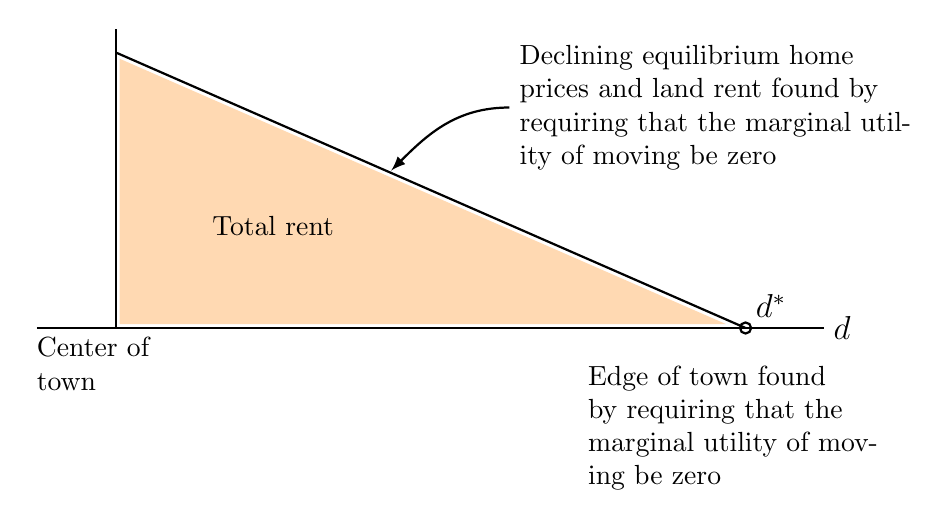
\begin{tikzpicture}[domain=0:2]
%\draw[thick,color=gray,step=.5cm, dashed] (-0.5,-.5) grid (3,3);
\draw[line width=.01] (0,0) -- (10,0) node[right] {\large $d$};
\node at (1,0) [below,text width=2cm] {Center of town};
%\draw[thick ] (0,3)node[above right] {merchant's price in town} -- (10,3) ;
\draw[thick ] (0,0)  -- (10,0); 
\draw[thick, -latex] (6,2.8)
node[right, text width=5cm]{Declining equilibrium  home prices and land rent found by requiring that the marginal utility of moving be zero} 
to [out=180, in=45](4.5,2); 

\fill[orange!30] (1.05,0.05)--(8.75,0.05)--(1.05,3.42)--cycle;

\draw[thick ] (1,0) -- (1,3.8);
\draw[thick ] (9,0)node [above right]{\large $d^*$}circle[radius=2pt] node[below=.35cm,text width=4cm] {Edge of town found by requiring that the marginal utility of moving be zero} -- (1,3.5) ;

\node at (3,1.3){Total rent};
\end{tikzpicture} 
\caption{Illustrating marginal and infra-marginal quantities with the bid-rent curve and aggregate rent.}
\label{fig-land-rent-as-inframarginal}
\end{figure}

In Figure~\ref{fig-land-rent-as-inframarginal}, The level of rent is determined at any distance by individuals making comparison locally. At point $d^*$ the person at the edge of the city decides whether to work in the centre or in the non-urban space. These are \gls{marginal} decisions. The orange area represents the total rents generated between $d=0$ and $d=d^*$. It is a summation of \textbf{\gls{inframarginal}} rents. Like Ricardo in his classic study \cite{ricardoEssayInfluenceLow1815}, we are concerned with the distribution of rents, which are an inframaginal quantity.


% \subsection{Coarse graining}

% Using agent based models, combined with simple equations is also one appraoch to coarse graining. 
% There's a distinction between coarse grained and fine grained models. Equation~\ref{eqn-population-output}  is a high-level generalization---a ``coarse-grained'' model. Modelling always faces a trade-off between computational tractability and representing details. \cite{GET_TerrysDissertation, GET_PaulsBook}

% Coarse-grained models must capture the stylized facts. %, as ours does.

% where the model is insenstitive to the details, you really want a representation that's small that captures the big pattern. 
% When you move to getting the details of the model, you know you have a model that tracks the observable. 
% Sometimes the model is sensitive to the details, and a more fine grained model is needed. There is an advantate to having a continuum of models that make it posible to represent systems with different levels of nuance/detail. We are focused on modelling a coarse grained model of the production system.
% % \section{SORT}
% % providing tractable models.  equilibrium analysis of marginal effects, and representative agents which hid distributional effects, as well as spaceless economic models of markets made it difficult to capture the richer spacial dynamics of urban rents, and the details of the ways economic forces play out for individual actors.

% % First they've not tended to build in, in a sophisticated way classical economic theory,
% % In general, classical economic theory has not been developed in agent-based modeling work
% % Agent-based models have begun with simple models, using and relaxing neoclassical assumptions, and building from first principles. This is absolutely the place to start. As the field matures, it makes sense to introduce theory in a more nuanced way, that connects with classical theory/the history of thought, etc

% % Second, relatively little agent-based modelling work integrates with the neoclassical economic work in a way that makes the relation clear/holds the advantages. ABM work tends to both reject neoclassical approaches and rely on neoclassical assumptions.
% % More generally only a few agent models (e.g. spruce budworm) connect the analytic and agent models in a clear rigorous way. We focus on holding in addition to the relation with classical theory, a close connection with the many advances made withing neoclassical modelling

% % - this connection will make it easier to incorporate in teaching and for mainstream economists to engage on and build with.

% % This work builds, first, a simple conceptually clear model tightly integrated with the core economic modelling traditions, that builds on the theory of rent.

% % ALSO (Agent modelling also tents to model individuals- we also take some steps to agent-based modelling beyond the individual, and to the work developing model in a mode ideas)

% % Third, econ lacks resilience analysis and models, yet hysteresis clearly present in the relation between the built environment and econ activity. Although there's been work on dynamics and individual effects, there has been little work looking at the resilience dynamics in economic models, we take that approach looking at the resilience of community and individual wealth, and the relationship between that wealth and productivity. 

% % - This puts resilience dynamics at the center of economic analysis.

% % The resilience analysis looks at the dynamics of rent in economic boom and bust cycles.
% % There is a ratchet effect, achieved through hysteresis in the system, in which sucks wealth out of communities on the way up and on the way down. % DETAIL ONCE DRAFTED.


% % The emphasis is on clarity and connecting with the equilibrium in economics, and systematically relaxing each, to connect with the analytic tradition of economic modelling
% % The clarity of intuition of the neoclassical tradition with the deeper root of distribution theory rooted in classical economics and the breath and rigor possible with new tools from the study of complexity and statistical physics.

\section{Summary}
In integrating models of the firm, the urban spatial system, the housing market and the financial system,  which are traditionally studied separately, this work combines elements of classical rent theory and neoclassical distribution theory with agent-based modeling. We have a spatially explicit agent-based land market model, an equilibrium urban rent model, a neoclassical equation-based model of urban production, and a rule-based mortgage provision system. It is not surprising that a work of this sort should draw on a variety of methodologies and should raise a range of somewhat subtle modeling issues. 

In this chapter, we have tried to make our solutions to certain high-level modeling questions explicit. We have at each point grounded our modeling decisions in familiar and accepted theory, while at the same time eliminating elements that would make our model unnecessarily complex. 